Per eliminare un progetto un utente deve essere iscritto ed autenticato. Per accedere alla pagina di eliminazione di un progetto l'utente deve premere il pulsante azzurro \textbf{My Project} posto in alto a destra sullo schermo. Una volta premuto si caricherà la pagina corrispondente. A questo punto l'utente deve selezionare il progetto da eliminare dalla lista dei progetti in alto a sinistra.
Una volta selezionato il progetto apparirà al centro dello schermo il titolo del progetto scelto,un'immagine di anteprima della prima slide del progetto e sotto a questa un menù. 

\begin{figure}[H] 
	\centering 
	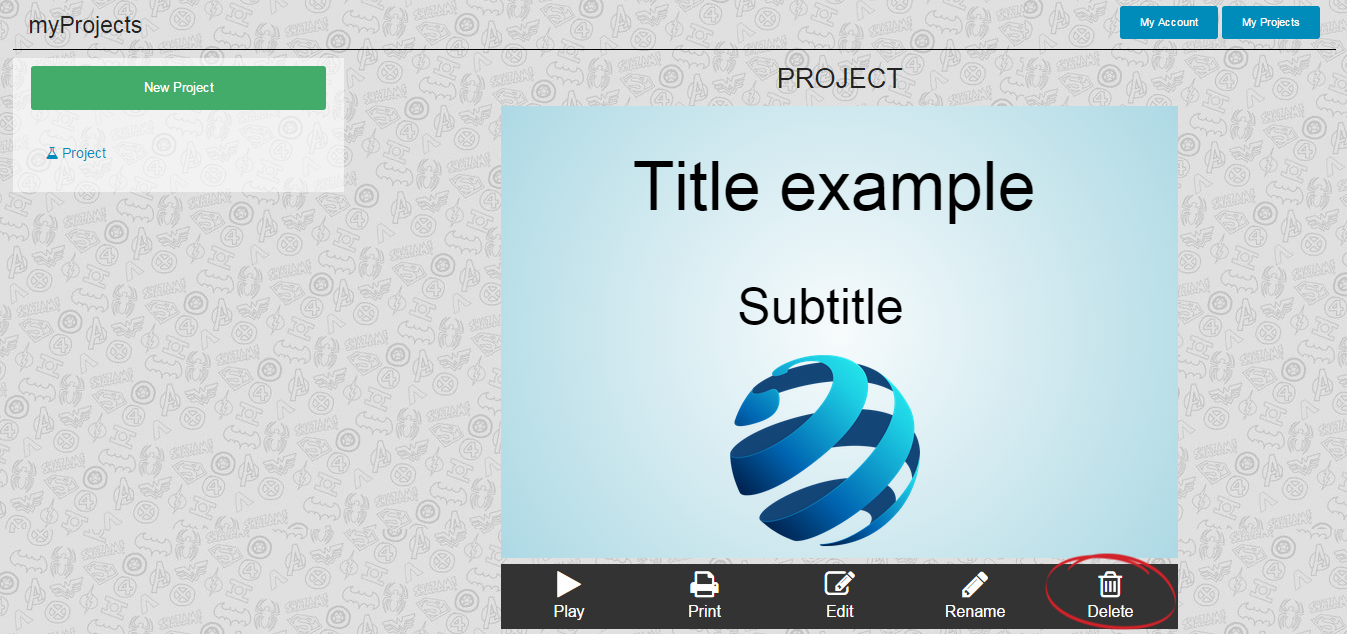
\includegraphics[scale=0.40] {img/elimina_pro.png}
	\caption{Eliminazione di un progetto} 
\end{figure}

Selezionando dal menù la voce \textbf{Delete} apparirà il seguente pop-up\ped{G}:

\begin{figure}[H] 
	\centering 
	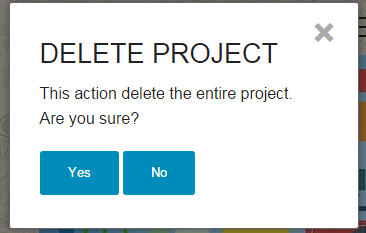
\includegraphics[scale=0.60] {img/del_project.png}
	\caption{Pop-up conferma eliminazione progetto} 
\end{figure}

\noindent Premendo il tasto \textbf{Yes} si confermerà l'eliminazione del progetto, premendo il tasto \textbf{No} il progetto non verrà eliminato.